\documentclass[a4paper,12pt]{article}

\usepackage[spanish]{babel}
\usepackage[utf8]{inputenc}
\usepackage[T1]{fontenc}
\usepackage{geometry}
\usepackage{graphicx}
\usepackage{amsmath}
\usepackage{setspace}
\usepackage{textcomp}
\usepackage[hidelinks]{hyperref}
\usepackage{enumitem}
\usepackage{fvextra}
\usepackage[most]{tcolorbox}
\usepackage{bm}
\usepackage{caption}
\usepackage{float}
\usepackage{placeins}

\geometry{margin=2.5cm}
\onehalfspacing

\setlist[itemize]{itemsep=0pt, topsep=6pt, parsep=0pt, partopsep=0pt}
\setlist[enumerate]{itemsep=0pt, topsep=6pt, parsep=0pt, partopsep=0pt}
\captionsetup{
    justification=centering,
    singlelinecheck=true
}

\begin{document}

\begin{titlepage}
\centering

Instituto Tecnológico de Buenos Aires\\
Trabajo Práctico Nº2\\
72.25 - Simulación de Sistemas\\[1cm]

{\LARGE Autómatas Celulares}\\[1cm]

Grupo: 5\\[0.5cm]

Integrantes:\\
Birsa Juan Pablo (64500)\\
jbirsa@itba.edu.ar\\
Gonzalez Cornet, Josefina (64550)\\
jgonzalezcornet@itba.edu.ar\\
Magri, Federico José (64508)\\
fmagri@itba.edu.ar\\[1cm]

Fecha de entrega: 30 de Marzo de 2026\\
1C - 2026

\end{titlepage}

\tableofcontents
\newpage

\newpage
\section{Introducción}

El presente trabajo práctico tiene como objetivo el estudio y la implementación computacional del modelo de bandadas para sistemas de partículas autopropulsadas, tomando como base el modelo introducido por T. Vicsek et al. (1995). Este sistema permite investigar la emergencia de movimiento ordenado y fenómenos colectivos presentes en la naturaleza, tales como bandadas de aves o bancos de peces. En estos sistemas, a partir de interacciones locales simples, se produce una transición de fase cinética continua desde un estado desordenado hacia un movimiento cooperativo macroscópico.

A diferencia del modelo estándar original, el aspecto central y novedoso de este proyecto es la incorporación de una partícula líder en el enjambre. El propósito de esta adición es analizar el impacto que tienen distintas geometrías de movimiento directriz sobre el grado de orden global del sistema al ser sometido a diferentes intensidades de ruido angular. De esta manera, el trabajo se enfoca en caracterizar la transición de fase y evaluar cómo la competencia entre las perturbaciones aleatorias y la presencia de un agente con trayectoria predefinida afecta la consolidación del movimiento colectivo.
\newpage
\section{Modelo}

\subsection{Sistema base sin líder}

El sistema base se define como un autómata celular de tipo off-lattice, el cual modela el comportamiento de bandadas de agentes autopropulsados. El sistema está compuesto por $N$ partículas puntuales que se desplazan de forma continua dentro de un dominio cuadrado de lado $L$, con condiciones periódicas de contorno.

La densidad del sistema se define como:

\begin{equation}
\rho = \frac{N}{L^2}
\end{equation}

por lo que, fijados $\rho$ y $L$, el número de partículas $N$ queda determinado.

La evolución temporal del sistema ocurre en pasos discretos de tiempo $\Delta t = 1$.

En cada iteración, la posición espacial del i-ésimo agente, denotada por el vector $\bm{x}_i(t)$, se actualiza a partir de su velocidad actual $\bm{v}_i(t)$ mediante:

\begin{equation}
\bm{x}_i(t+1) = \bm{x}_i(t) + \bm{v}_i(t)
\end{equation}

El módulo de la velocidad $v$ de todas las partículas es constante e igual a lo largo de toda la simulación.

La dirección del movimiento de cada partícula, definida por el ángulo $\theta_i(t+1)$, se actualiza en cada paso temporal según:

\begin{equation}
\theta_i(t+1) = \langle \theta(t) \rangle_{r_c} + \Delta \theta
\end{equation}

donde $\langle \theta(t) \rangle_{r_c}$ representa la dirección promedio de las partículas (incluyendo a la propia partícula $i$) que se encuentran dentro de un radio de interacción $r_c$.

Este promedio se calcula a partir de las componentes trigonométricas de las direcciones de las partículas vecinas.

Por su parte, el término $\Delta \theta$ introduce ruido en el sistema, actuando como un parámetro análogo a la temperatura. Este se define como una variable aleatoria con distribución uniforme en el intervalo $[-\eta/2,\eta/2]$, donde $\eta$ controla la intensidad de la perturbación angular.

\subsection{Escenario con partícula líder}

A diferencia del modelo estándar, en los escenarios con líder se introduce una partícula particular dentro de la celda de simulación. La característica principal de esta partícula es que su movimiento está predefinido matemáticamente y no se ve alterado por la interacción con las partículas vecinas. No obstante, el líder sí influye sobre las partículas regulares, ya que estas lo contabilizan dentro de su radio de interacción $r$ al calcular su propio ángulo promedio $\langle \theta(t) \rangle_r$.

Para el presente estudio, se evalúan dos geometrías de movimiento predefinidas para la partícula líder:

\begin{itemize}
\item Líder con dirección fija: La partícula posee una dirección de movimiento constante a lo largo de todo el tiempo, la cual se asigna de manera aleatoria al inicio de la simulación.
\item Líder con trayectoria circular: La partícula describe una trayectoria circular prefijada de radio $R=5$ alrededor de un centro arbitrario. Su velocidad angular se ajusta de manera tal que el módulo de su velocidad tangencial sea equivalente a la velocidad escalar $v$ del resto de las partículas del sistema.
\end{itemize}

\subsection{Observable de interés}

Para medir el comportamiento general del enjambre y analizar la transición de fase al variar el ruido $\eta$ o la densidad $\rho$, es necesario definir un parámetro de orden. En este modelo, el observable principal es la polarización, denotada por $v_a$, que mide el grado de alineamiento colectivo del sistema.

Este parámetro se define como:

\begin{equation}
v_a = \frac{1}{N v} \left| \sum_{i=1}^{N} \bm{v}_i \right|
\end{equation}

donde $N$ es el número total de partículas y $v$ es el módulo constante de la velocidad individual.

El observable $v_a$ toma valores cercanos a 0 cuando las direcciones de las partículas están distribuidas de manera aleatoria, lo que corresponde a un estado desordenado. En cambio, valores cercanos a 1 indican un alto grado de alineamiento, característico de un estado ordenado.

\newpage
\section{Implementación}

\subsection{Arquitectura y Módulos}

El modelo se implementó en Java 21. Posteriormente, para la generación de animaciones y gráficos se utilizó Python 3. El proyecto se estructura de la siguiente manera:

\begin{center}
\begin{minipage}{0.55\textwidth}
\begin{Verbatim}
tp2-code/
|__ Particle.java
|__ Leader.java
|__ FixedLeader.java
|__ CircularLeader.java
|__ CellIndexMethod.java
|__ VicsekModel.java
|__ Generator.java
|__ Main.java
|__ OutputWriter.java
tp2-visual/
|__ visualizer.py
|__ graphs.py
\end{Verbatim}
\end{minipage}
\end{center}

La arquitectura de la implementación implica las siguientes responsabilidades:

\begin{itemize}
\item Particle.java: modela la estructura interna de una partícula.
\item Leader.java: clase abstracta creada por buenas prácticas de programación orientada a objetos.
\item FixedLeader.java: modela la estructura del líder con dirección fija.
\item CircularLeader.java: modela la estructura del líder con trayectoria circular.
\item CellIndexMethod.java: implementa el método utilizado por el VicsekModel para el cálculo de vecinos, los cuales influyen en la trayectoria de determinada partícula.
\item VicsekModel.java: implementación del modelo de Vicsek. Recibe por parámetro los valores necesarios para la simulación.
\item Generator.java: genera las partículas en ubicaciones aleatorias con ángulos aleatorios. En caso de haber líder, también lo crea.
\item Main.java: permite ejecutar corridas completas de la simulación. Incluye la definición de los parámetros. Calcula todos los valores necesarios adicionales para el análisis posterior.
\item OutputWriter.java: realiza la escritura de los archivos .txt de output requeridos.
\item visualizer.py: realiza las animaciones correspondientes basadas en los archivos .txt generados por OutputWriter.java.
\item graphs.py:
\end{itemize}

\subsection{Algoritmo}

Para la simulación computacional, la actualización de las posiciones y ángulos definidos en el modelo matemático se traduce en el procedimiento descrito en el Algoritmo 1. 
Para optimizar la búsqueda de partículas vecinas dentro del radio de interacción $r_c$, se reutilizó la implementación del método de Cell Index desarrollada en el Trabajo Práctico N°1. Este método devuelve, para cada partícula, una lista con los índices de aquellas que se encuentran en su vecindad, obteniendo así una estructura de datos eficiente donde a cada agente i se le asocia el conjunto de sus vecinos interactuantes.

\begin{center}
\begin{tcolorbox}[width=0.9\textwidth, colback=white, colframe=black, boxrule=0.6pt]
\begin{enumerate}
    \item Identificación de vecinos dentro del radio de interacción $r_c$ mediante el método de Cell Index, reutilizando la implementación desarrollada en el Trabajo Práctico N°1.
    \item Cálculo del ángulo promedio de las partículas vecinas.
    \item Incorporación de un término de ruido uniforme $\Delta \theta$.
    \item Actualización de direcciones y posiciones, aplicando condiciones periódicas de contorno.
\end{enumerate}
\end{tcolorbox}
\small{Algoritmo 1: Paso de simulación, modelo de Vicsek}
\end{center}

\subsection{Formato de Datos y Reproducibilidad}

El resultado de cada ejecución de la simulación se vuelca en un archivo output.xyz. Este formato resulta útil porque permite su uso en distintas herramientas de visualización, facilitando el análisis y la exploración de la dinámica del sistema de manera más intuitiva.

Este almacena la información de todos los pasos temporales simulados de la siguiente manera:

\begin{center}
\begin{tcolorbox}[width=0.8\textwidth, colback=white, colframe=black, boxrule=0.6pt]
\begin{Verbatim}
N L rho v rc eta steps leaderType
step i
id_particula pos_x pos_y vel_x vel_y is_leader
step i+1
id_particula pos_x pos_y vel_x vel_y is_leader
...
\end{Verbatim}
\end{tcolorbox}
\end{center}

donde:

Primero se indican los parámetros utilizados en la simulación:

\begin{itemize}
\item $N$ indica el número de partículas en la simulación.
\item $L$ indica la longitud del lado del dominio cuadrado de simulación.
\item $\rho$ indica la densidad de partículas.
\item $v$ indica la velocidad de las partículas.
\item $r_c$ indica el radio de interacción entre partículas.
\item $\eta$ indica el nivel de ruido.
\item steps indica la cantidad total de pasos temporales simulados.
\item leaderType indica en qué caso se encuentra: sin líder, con líder de dirección fija o con líder de trayectoria circular.
\end{itemize}

Luego se provee el detalle step a step del modelo:

\begin{itemize}
\item step $i$ indica el número de paso descrito a continuación.
\item id\_particula es un número entero que identifica a las partículas.
\item pos\_x indica la posición en X de la partícula correspondiente.
\item pos\_y indica la posición en Y de la partícula correspondiente.
\item vel\_x indica la componente en X de la velocidad de la partícula correspondiente.
\item vel\_y indica la componente en Y de la velocidad de la partícula correspondiente.
\item is\_leader es una opción binaria utilizada para la distinción del líder entre las partículas.
\end{itemize}

\newpage
\section{Simulaciones}

\subsection{Parámetros fijos}

Para todas las simulaciones se utilizaron los siguientes parámetros:

\begin{itemize}
\item $L=10$: longitud del lado del dominio cuadrado de simulación
\item $\rho=4$: densidad de partículas
\item $N=400$: número total de partículas
\item $v=0.03$: velocidad de las partículas
\item $r_c=1$: radio de interacción
\item $dt=1$: paso temporal
\end{itemize}

\subsection{Parámetros variables}

Se variaron los siguientes parámetros:

\begin{itemize}
\item $\eta$ (ruido): valores en el intervalo $[0.1, 5]$
\item $\rho$ (densidad): además del valor principal $\rho=4$, se consideraron $\rho=2$ y $\rho=8$.
\item steps: cantidad de pasos temporales, ajustada según el análisis requerido en cada caso.
\end{itemize}

\subsection{Diseño experimental}

El diseño experimental contempló simulaciones independientes para las tres configuraciones de liderazgo definidas previamente en la Sección 2.2.

Para caracterizar el comportamiento inicial del sistema, se realizaron simulaciones utilizando valores representativos del ruido ($\eta$=0.1, 1, 3), manteniendo fija la densidad en $\rho=4$. En estos casos, se utilizaron los pasos temporales suficientes que permitieran analizar la evolución de la bandada y su relajación. A partir de estas simulaciones se estudió la evolución temporal de la polarización. El observable escalar se calculó promediando la polarización exclusivamente durante el régimen estacionario, cuyo criterio cuantitativo de inicio y descarte del transitorio inicial se encuentra detallado en la Sección 5.1.

Adicionalmente, se realizaron 50 ejecuciones independientes para distintos valores del ruido $\eta$, con el fin de obtener la polarización $v_a$ promedio y estimar su variabilidad estadística frente a las fluctuaciones.

Finalmente, se llevaron a cabo simulaciones adicionales para $\rho=2$ y $\rho=8$, con el objetivo de analizar el efecto específico de la densidad sobre la polarización macroscópica y la dinámica grupal del sistema.

\newpage
\section{Resultados}

Los resultados obtenidos a partir de las simulaciones se presentan y analizan a continuación.

\subsection{Evolución temporal del observable}

En las Fig. 1, Fig. 2 y Fig. 3 expuestas a continuación se presentan las evoluciones temporales de la polarización ($v_a$) correspondientes a las tres condiciones experimentales detalladas previamente. En cada una de estas figuras se realiza una superposición de tres valores del parámetro de ruido ($\eta = 0.1$, $\eta = 1$ y $\eta = 3$), permitiendo un análisis comparativo directo del impacto del ruido en la dinámica del sistema para cada caso de estudio. Estas representaciones gráficas tienen como propósito fundamental justificar la selección de la ventana temporal de medición. Al observar la convergencia de las curvas, se establecen los criterios para identificar el inicio del estado estacionario, garantizando que el promedio del observable ($v_a$) se realice sobre un intervalo donde las fluctuaciones se han estabilizado y el transitorio inicial ha sido superado.

Para determinar el instante de inicio del estado estacionario ($t_0$) en cada configuración, se estableció un criterio cuantitativo basado en la estabilidad de las fluctuaciones del observable ($v_a$). Se definió una banda de tolerancia específica para cada caso; el estado estacionario se considera alcanzado en el momento en que cinco mediciones consecutivas de la polarización presentan variaciones relativas inferiores a dicha tolerancia. En aquellos casos donde las fluctuaciones inherentes al sistema impiden que se cumpla esta condición antes de transcurrir el 40\% de la simulación, se adopta de manera conservadora este límite temporal ($t_0=0.4T$) como el inicio del régimen estacionario, garantizando así la exclusión del período transitorio inicial.

% FIGURA 1
\begin{figure}[h]
\centering
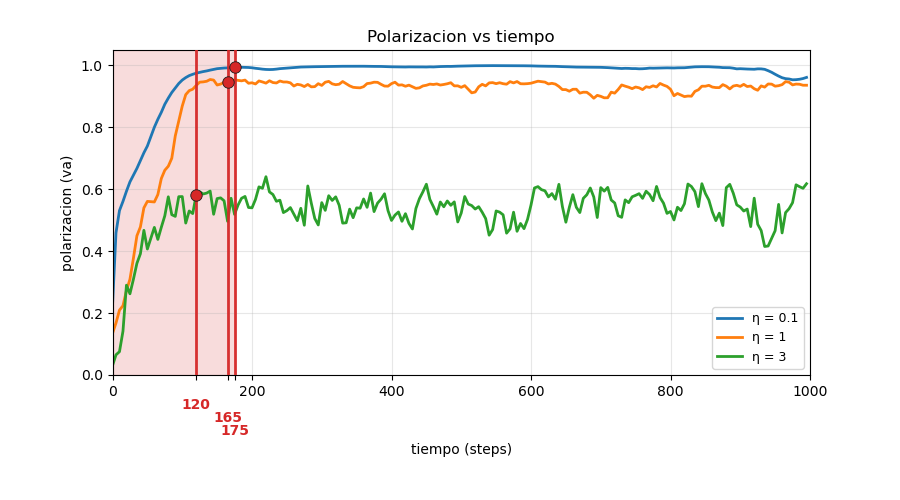
\includegraphics[width=0.8\textwidth]{figuras/figura1.png}
\caption{Evolución de la polarización con respecto al tiempo, sin una partícula líder.}
\end{figure}

En la Fig. 1 se presenta la evolución de la polarización en función del tiempo para el escenario base sin partícula líder. Aplicando el criterio descrito, las tolerancias determinadas empíricamente fueron de 0.001 para el caso de bajo ruido ($\eta=0.1$), 0.008 para un ruido intermedio ($\eta=1$) y 0.05 para la simulación con ruido elevado ($\eta=3$). Estos umbrales crecientes reflejan cómo la amplitud de las fluctuaciones naturales del enjambre se magnifica a medida que se incrementa el ruido del sistema.

% FIGURA 2
\begin{figure}[h]
\centering
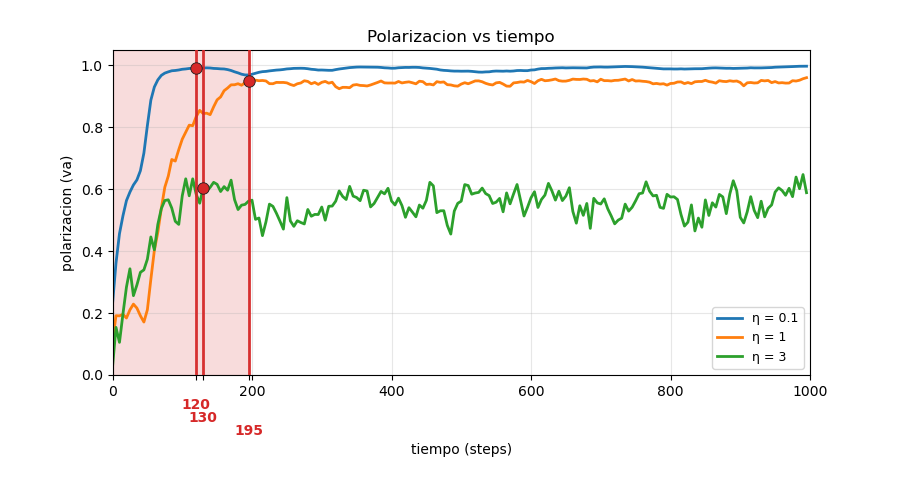
\includegraphics[width=0.8\textwidth]{figuras/figura2.png}
\caption{Evolución de la polarización con respecto al tiempo, con una partícula líder con dirección fija.}
\end{figure}

De manera análoga, la Fig. 2 exhibe el comportamiento temporal para el escenario que incorpora un líder con dirección fija. Para esta configuración, las tolerancias requeridas para identificar el estado estacionario fueron de 0.001, 0.002 y 0.03 para los niveles de ruido $\eta=0.1$, $\eta=1$ y $\eta=3$, respectivamente. Se puede notar que, ante ruidos moderados e intensos, los umbrales de fluctuación son ligeramente menores que en el caso base, sugiriendo que la presencia de una partícula directriz constante contribuye a estabilizar el movimiento del grupo más rápidamente.

% FIGURA 3
\begin{figure}[h]
\centering
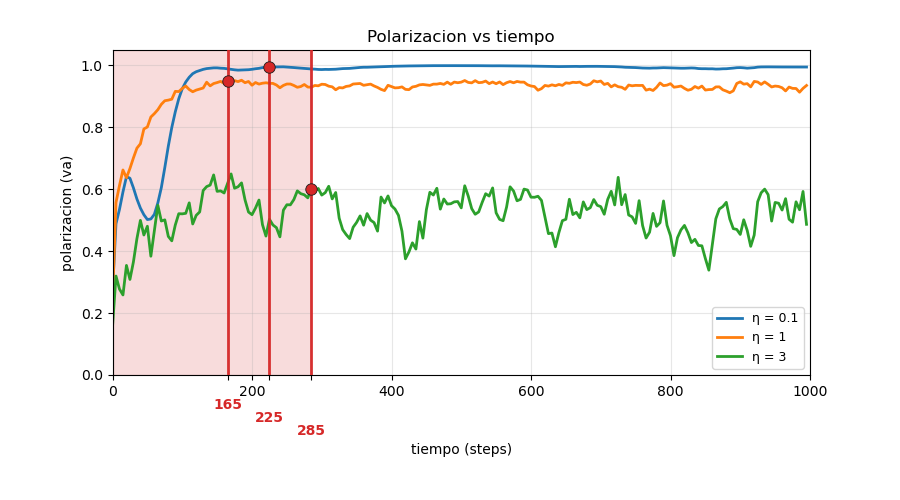
\includegraphics[width=0.8\textwidth]{figuras/figura3.png}
\caption{Evolución de la polarización con respecto al tiempo, con una partícula líder con trayectoria circular.}
\end{figure}

Finalmente, en la Fig. 3 se detalla la evolución correspondiente al sistema regido por un líder de trayectoria circular. Las tolerancias establecidas para capturar la estabilización de $v_a$ en este tercer escenario fueron de 0.001, 0.0045 y 0.025 para $\eta=0.1$, $\eta=1$ y $\eta=3$, respectivamente. Al igual que en las condiciones anteriores, la dispersión temporal del parámetro de orden muestra una dependencia directa con la intensidad de la perturbación angular $\eta$.

\subsection{Relación entre el ruido del sistema y el observable}

En las Fig. 4, Fig. 5 y Fig. 6 se presenta la dependencia del observable $v_a$ con el parámetro de ruido $\eta$ para cada una de las condiciones de liderazgo consideradas. En todos los casos, para valores bajos de $\eta$, la polarización se mantiene cercana a 1, indicando un alto grado de alineamiento colectivo entre las partículas.

A medida que el ruido aumenta, se observa una disminución progresiva de $v_a$, lo que refleja la pérdida de coherencia en el movimiento. Esta evolución evidencia una transición continua desde un estado ordenado hacia uno desordenado, en concordancia con el comportamiento esperado del modelo de Vicsek. Para valores elevados de $\eta$, la polarización tiende a cero, caracterizando un régimen dominado por el ruido.

Cada punto de las curvas corresponde al promedio de 50 ejecuciones independientes, mientras que las barras de error representan el desvío entre dichas ejecuciones, proporcionando una medida de la dispersión del observable.

% FIGURA 4
\begin{figure}[H]
\centering
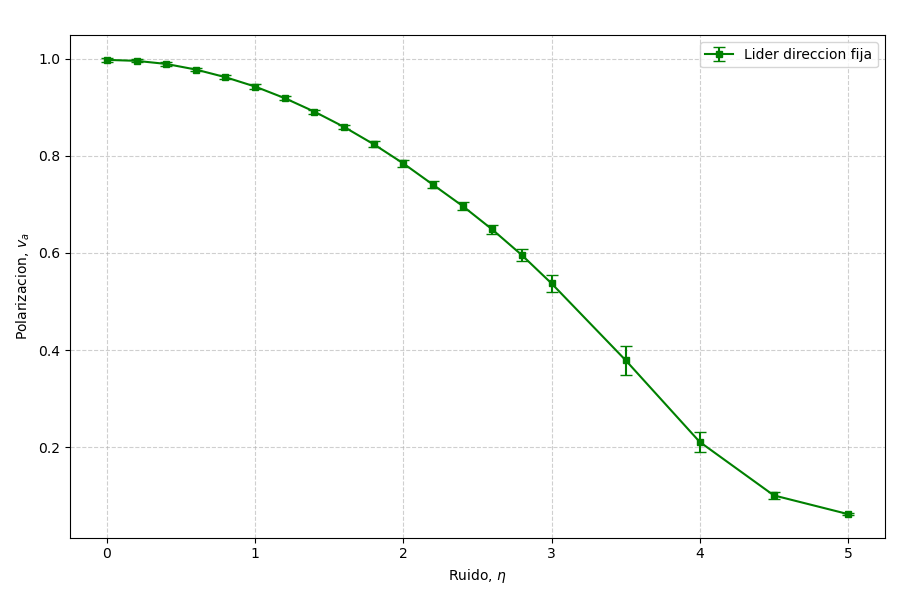
\includegraphics[width=0.8\textwidth]{figuras/figura4.png}
\caption{Polarización en función del ruido para un sistema sin partícula líder.}
\end{figure}

% FIGURA 5
\begin{figure}[H]
\centering
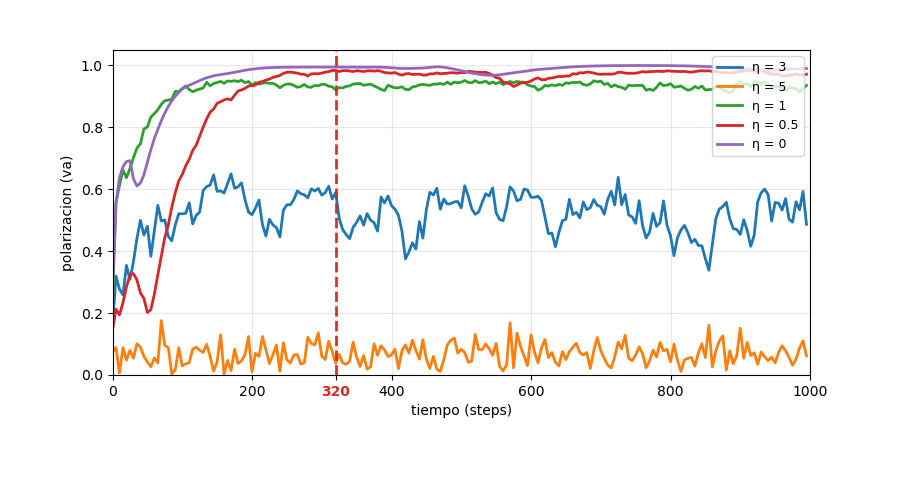
\includegraphics[width=0.8\textwidth]{figuras/figura5.png}
\caption{Polarización en función del ruido para un sistema con líder de dirección fija.}
\end{figure}

% FIGURA 6
\begin{figure}[H]
\centering
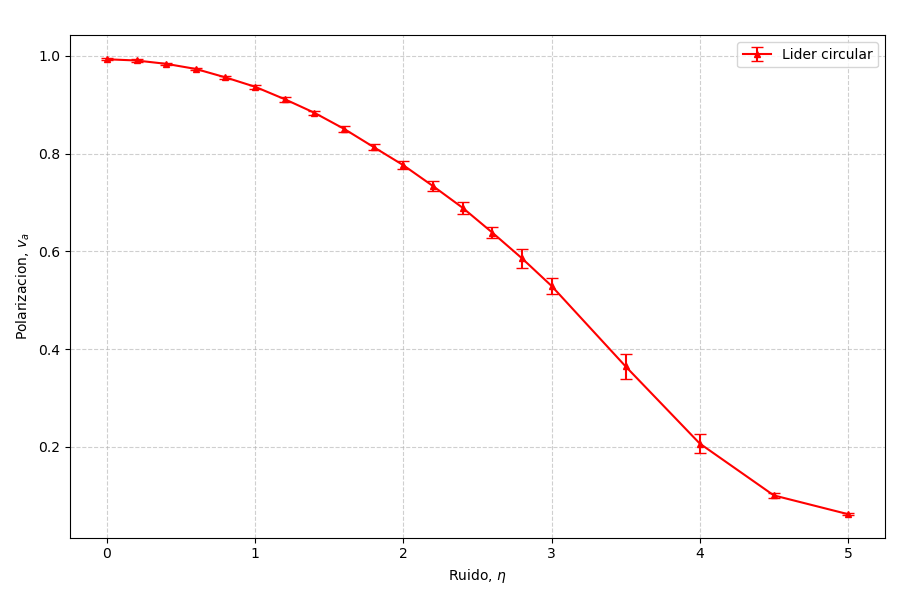
\includegraphics[width=0.8\textwidth]{figuras/figura6.png}
\caption{Polarización en función del ruido para un sistema con líder circular.}
\end{figure}

\FloatBarrier

\subsection{Comparativa entre escenarios con distintos líderes}

En la Fig. 7 se contrastan los resultados obtenidos para las tres condiciones experimentales consideradas: sistema sin líder, sistema con líder de dirección fija y sistema con líder de trayectoria circular, con el objetivo de analizar la influencia de la geometría del movimiento del líder sobre el grado de orden del sistema.

Si bien las tres configuraciones presentan un comportamiento global similar, se observan diferencias en valores intermedios del ruido. En particular, el sistema con líder de dirección fija tiende a exhibir valores de polarización levemente superiores, lo cual es consistente con una mayor capacidad para sostener el alineamiento colectivo frente a perturbaciones.

En contraste, el escenario con líder de trayectoria circular presenta, en general, valores ligeramente menores de polarización, posiblemente asociado a la variabilidad de su dirección de movimiento, introduciendo una perturbación adicional en la dinámica del sistema.

No obstante, las diferencias observadas se encuentran dentro del orden de magnitud de las barras de error, lo que indica que el impacto del tipo de liderazgo sobre la polarización global es limitado en comparación con la influencia dominante del ruido.

% FIGURA 7
\begin{figure}[H]
\centering
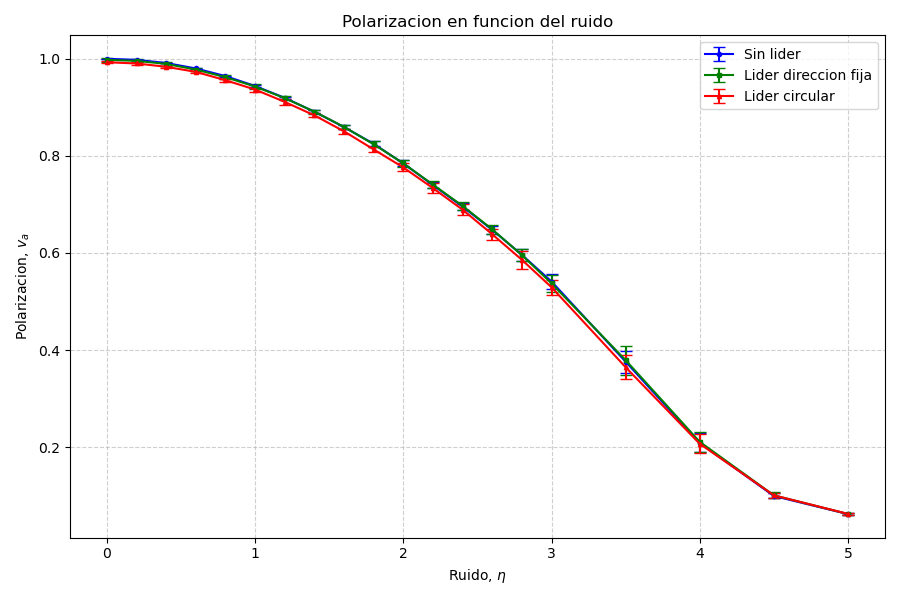
\includegraphics[width=0.8\textwidth]{figuras/figura7.png}
\caption{Polarización en función del ruido para los tres sistemas.}
\end{figure}

\FloatBarrier

\subsection{Influencia de la densidad}

Con el objetivo de analizar el efecto de la densidad sobre el comportamiento del sistema, se realizaron simulaciones adicionales para $\rho=2$ y $\rho=8$, considerando distintos valores del parámetro de ruido. Para este análisis detallado, se tomó como caso de estudio el escenario del sistema base sin líder.

A nivel macroscópico, los resultados obtenidos muestran un comportamiento cualitativamente similar al caso base $\rho=4$, observándose en todos los casos una transición desde un estado ordenado hacia uno desordenado a medida que aumenta el ruido. No obstante, se identifican diferencias en la dinámica del sistema asociadas a la densidad.

Para determinar el inicio del régimen estacionario en estos nuevos escenarios, se aplicó el mismo criterio cuantitativo de estabilidad de fluctuaciones previamente descrito, evaluando las evoluciones temporales de forma independiente. En la Fig. \ref{fig:densidad2_01} y la Fig. \ref{fig:densidad2_3} se observa el comportamiento de la polarización para el sistema menos denso ($\rho=2$) sometido a un ruido bajo ($\eta=0.1$) y a un ruido elevado ($\eta=3$), respectivamente. Para estos casos, se determinaron empíricamente tolerancias de 0.001 y 0.03.

% FIGURA 8
\begin{figure}[H]
\centering
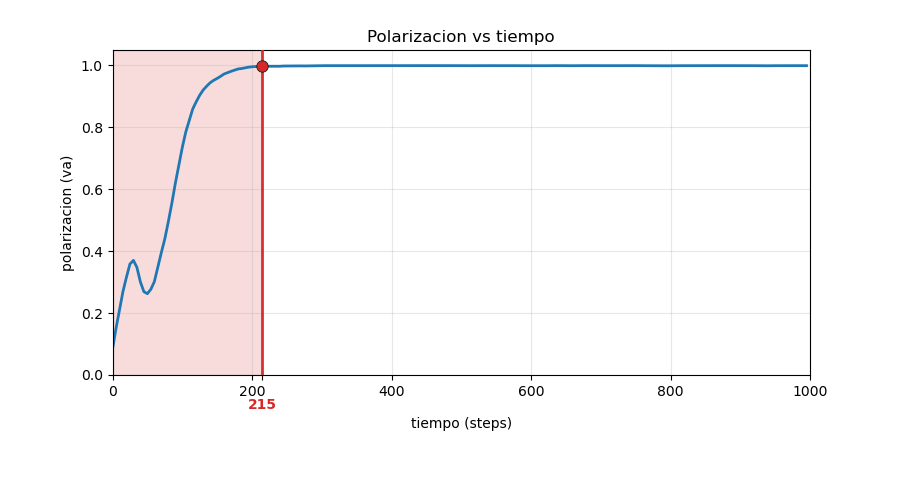
\includegraphics[width=0.8\textwidth]{figuras/figura8.png}
\caption{Polarización vs tiempo para $\rho=2$, $\eta=0.1$.}
\label{fig:densidad2_01}
\end{figure}

% FIGURA 9
\begin{figure}[H]
\centering
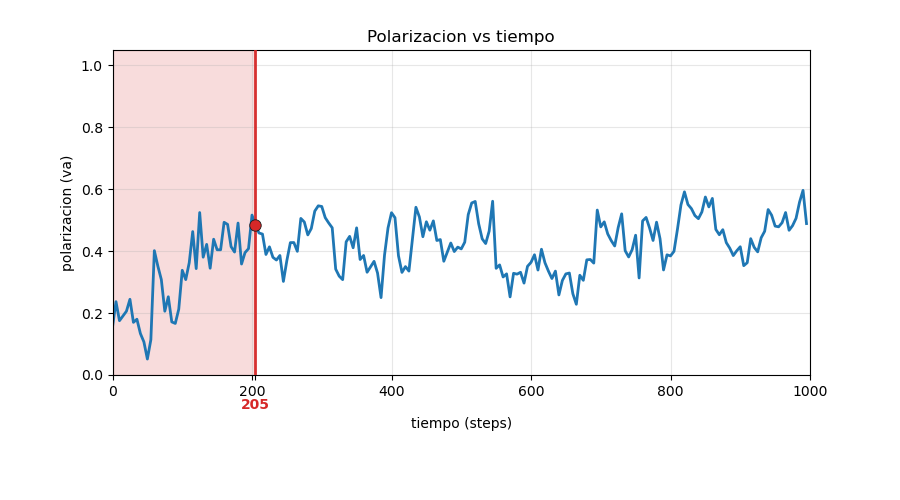
\includegraphics[width=0.8\textwidth]{figuras/figura9.png}
\caption{Polarización vs tiempo para $\rho=2$, $\eta=3$.}
\label{fig:densidad2_3}
\end{figure}

Por otro lado, la Fig. \ref{fig:densidad8_01} y la Fig. \ref{fig:densidad8_3} exhiben la evolución temporal del observable al incrementar la densidad del sistema ($\rho=8$) para los mismos niveles de ruido ($\eta=0.1$ y $\eta=3$), requiriendo tolerancias de 0.001 y 0.02.

% FIGURA 10
\begin{figure}[H]
\centering
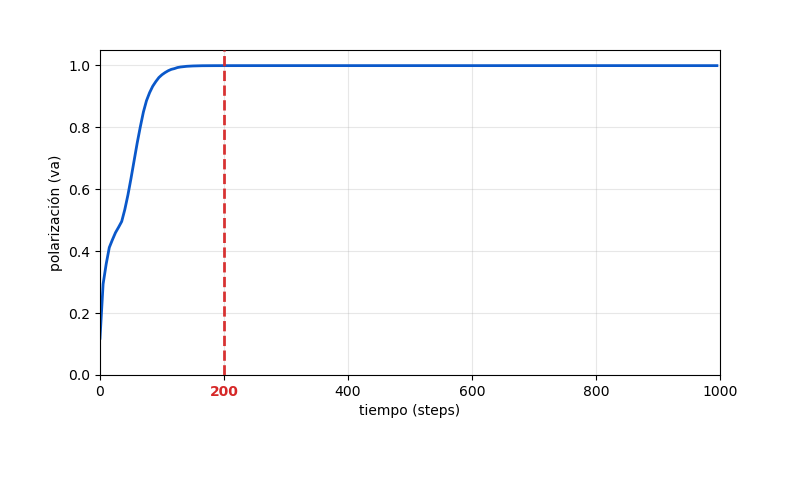
\includegraphics[width=0.8\textwidth]{figuras/figura10.png}
\caption{Polarización vs tiempo para $\rho=8$, $\eta=0.1$.}
\label{fig:densidad8_01}
\end{figure}

% FIGURA 11
\begin{figure}[H]
\centering
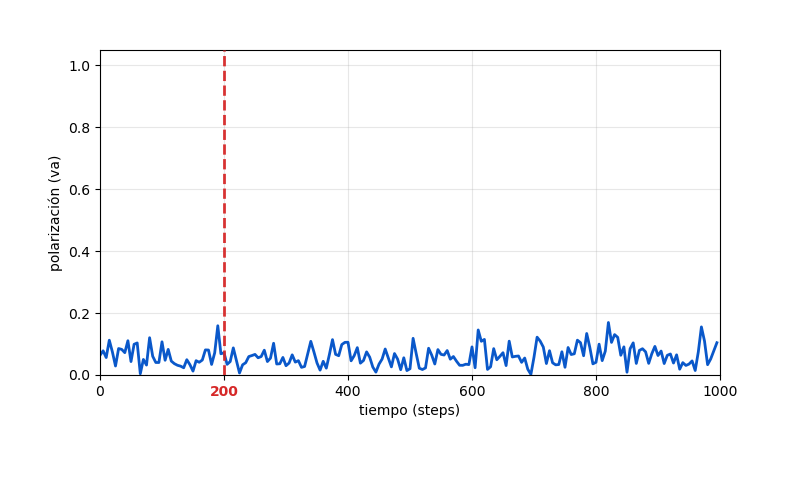
\includegraphics[width=0.8\textwidth]{figuras/figura11.png}
\caption{Polarización vs tiempo para $\rho=8$, $\eta=3$.}
\label{fig:densidad8_3}
\end{figure}

Es notable cómo, ante el mismo nivel de ruido elevado ($\eta=3$), el sistema más denso presenta un umbral de fluctuación menor (0.02 frente a 0.03). Esto confirma que una mayor cantidad de partículas por unidad de área contribuye a mitigar la dispersión del observable $v_a$.

Para ilustrar gráficamente la marcada dispersión y la dificultad de alcanzar un orden global en sistemas poco densos con perturbaciones elevadas, la Fig. \ref{fig:animacion_densidad} presenta una captura de la configuración espacial correspondiente al escenario con $\rho=2$ y $\eta=3$.

% FIGURA 12
\begin{figure}[H]
\centering
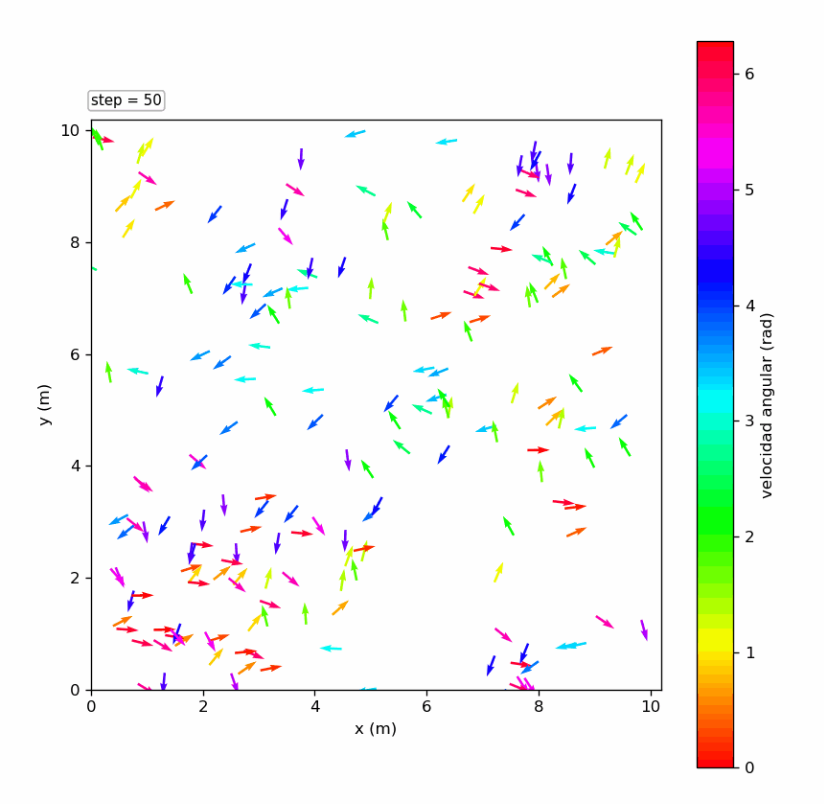
\includegraphics[width=0.8\textwidth]{figuras/figura12.png}
\caption{Configuración espacial para $\rho=2$, $\eta=3$.}
\label{fig:animacion_densidad}
\end{figure}

En esta imagen se evidencia cómo la reducción en la cantidad total de partículas incrementa significativamente la distancia media entre ellas, lo que disminuye la probabilidad de encontrar vecinos dentro del radio de interacción $r_c$. Esto provoca que el sistema se encuentre muy disperso, formando únicamente grupos polarizados pequeños e inestables que son rápidamente desarmados por el ruido, impidiendo que el enjambre consolide una dirección de movimiento unificada.

Por el contrario, para densidades elevadas, la interacción colectiva entre partículas adquiere mayor relevancia. En este caso, el aumento de las interacciones locales permite que el sistema logre mantener una polarización $v_a$ más elevada y estable, mitigando eficazmente el efecto desestabilizador ante niveles altos de ruido $\eta$.
\clearpage
\section{Conclusiones}

En el presente trabajo se implementó y analizó el modelo de Vicsek para sistemas de partículas autopropulsadas, incorporando una partícula líder con distintas geometrías de movimiento. A partir de las simulaciones realizadas, se estudió el comportamiento del sistema en función del parámetro de ruido $\eta$ y de la densidad $\rho$, evaluando su impacto sobre el grado de orden colectivo medido mediante la polarización.

Los resultados obtenidos evidencian que el ruido constituye el principal factor en la dinámica del sistema, determinando la transición continua desde un estado ordenado, caracterizado por un alto alineamiento entre partículas, hacia un régimen desordenado en el que las direcciones de movimiento se distribuyen de manera aleatoria. Este comportamiento se observa de manera consistente en todas las configuraciones consideradas.

En cuanto a la influencia de la partícula líder, se encontró que su efecto sobre la polarización global es prácticamente nulo en comparación con el impacto dominante del ruido. Al contrastar los escenarios con líder de dirección fija y líder de trayectoria circular, no se observan diferencias en el grado de orden; las curvas de polarización resultan virtualmente idénticas a la del sistema base y cualquier mínima variación se encuentra dentro del orden de magnitud de las barras de error y las fluctuaciones naturales del sistema.

Por otro lado, el análisis de la densidad revela que su efecto es fundamental para la consolidación del movimiento cooperativo. En sistemas de baja densidad, la gran distancia media entre partículas dificulta la propagación de la información, resultando en un enjambre altamente disperso e incapaz de mantener el consenso. Esto se hace evidente en el escenario sin líder al observar la Fig. 9, donde para un ruido elevado ($\eta$=3) y una baja densidad ($\rho$=2), la polarización sufre fluctuaciones severas y caóticas. Por el contrario, tal como refleja la Fig. 11 para el mismo escenario bajo el mismo nivel de ruido pero con una densidad elevada ($\rho$=8), el enjambre logra atenuar estas perturbaciones y estabilizarse notablemente. En este sentido, una mayor densidad $\rho$ favorece el orden colectivo: al aumentar las interacciones locales, el sistema logra mantener una polarización $v_a$ más elevada y estable, mitigando el efecto ante niveles altos de ruido $\eta$.

En conjunto, los resultados muestran que el comportamiento macroscópico del sistema surge de la competencia directa entre el ruido y las interacciones locales promovidas por la densidad, siendo el ruido el principal determinante del grado de desorden, mientras que la presencia y geometría de una partícula líder resulta tener un impacto marginal sobre el orden colectivo global.

\newpage
\section*{Referencias}

[1] Vicsek, T., et al. ``Novel type of phase transition in a system of self-driven particles'', Physical Review Letters, 1995.

\end{document}
